\documentclass[11pt,a4paper]{article}
\usepackage[T1]{fontenc}
\usepackage[utf8]{inputenc}
\usepackage{lmodern}
\usepackage{textcomp}
\usepackage[left=1.8cm,right=1.8cm,top=2.3cm,bottom=2.2cm,headheight=14pt,headsep=8pt]{geometry}
\usepackage{multicol}
\usepackage{xcolor}
\usepackage{fancyhdr}
\usepackage{graphicx}
\usepackage{array}
\usepackage{amsmath,amssymb}
\usepackage{setspace}
\usepackage{longtable}
\graphicspath{{../}}
\definecolor{ygreen}{RGB}{46,139,87}
\renewcommand{\normalsize}{\fontsize{10.9}{13.4}\selectfont}
\renewcommand{\familydefault}{\rmdefault}
\setlength{\parindent}{0pt}
\setlength{\columnsep}{0.8cm}
\setlength{\columnseprule}{0.4pt}
\setlength{\multicolsep}{3pt plus 1pt minus 1pt}
\renewcommand{\textsubscript}[1]{\ensuremath{_{\text{\fontsize{8}{8}\selectfont #1}}}}
\renewcommand{\textsuperscript}[1]{\ensuremath{^{\text{\fontsize{8}{8}\selectfont #1}}}}
\newcommand{\diqqat}[1]{\par\smallskip\noindent\textbf{Diqqat!} #1\par\medskip}
\newcommand{\javob}{\par\smallskip\noindent\textbf{Javob:} \rule[-2pt]{7.5cm}{0.4pt}\par\smallskip\noindent\textbf{Diqqat!} Javobingizni javoblar varaqasiga ko`chirib yozing.\par\medskip}
\pagestyle{fancy}
\fancyhf{}
\renewcommand{\headrulewidth}{0.4pt}
\fancyhead[L]{\textit{Milliy sertifikat 2026. Kimyo}}
\fancyhead[R]{1-variant}
\fancyfoot[L]{\fontsize{8}{9}\selectfont \textcopyright{} Colba maktabi, 2026}
\fancyfoot[C]{\thepage}
\fancypagestyle{first}{\fancyhf{}\renewcommand{\headrulewidth}{0pt}\fancyfoot[L]{\fontsize{8}{9}\selectfont \textcopyright{} Colba maktabi, 2026}\fancyfoot[C]{\thepage}}
\begin{document}
\normalsize
\thispagestyle{first}
\noindent\fcolorbox{ygreen}{white}{\parbox{\dimexpr\linewidth-2\fboxsep-2\fboxrule\relax}{%
\textbf{\fontsize{13}{15}\selectfont Nazorat testi}\ \textit{\fontsize{10}{12}\selectfont $\cdot$ Aralash test $\cdot$ 1-variant}\hfill
\begin{tabular}[t]{@{}r@{}}\textit{Milliy sertifikat 2026. Kimyo}\\ \textbf{\textit{\fontsize{8}{9}\selectfont Vaqt:}} \textit{\fontsize{10}{12}\selectfont 180 daqiqa}\end{tabular}}}
\par\medskip
\noindent\textit{Davriy jadvaldan foydalanish mumkin.}
\par\medskip
\begin{multicols}{2}
\noindent\textbf{1.} 11,2 g temir mo`l xlor bilan to`liq reaksiyaga kirishib, 32,5 g tuz hosil qildi. Sarflangan xlorning \textbf{hajmini (l, n.sh.) aniqlang.}

\noindent A)~\textsl{4,48} \hfill B)~\textsl{6,72} \hfill C)~\textsl{8,96} \hfill D)~\textsl{3,36}\par
\vspace{4pt}
\noindent\textbf{2.} Tarozining chap pallasida 35 g mis va 28 g kalsiy metallari bor. Misning ma'lum bir qismi va massa bo`yicha 25\% ko`proq kalsiy ajratib olinib, oksidlandi. Qolgan metall bo`laklari tarozining chap pallasiga, hosil bo`lgan oksidlar o`ng pallasiga joylashtirildi va tarozi muvozanatga keldi. Oksidlash uchun olingan mis bo`lagining \textbf{massasini (g) aniqlang.}

\noindent A)~\textsl{10} \hfill B)~\textsl{12} \hfill C)~\textsl{15} \hfill D)~\textsl{8}\par
\vspace{4pt}
\noindent\textbf{3.} Sirka kislota va etanol o`zaro ta'sirlashganda (H\textsubscript{2}SO\textsubscript{4} ishtirokida) hosil bo`lgan murakkab efir molekulasi tarkibidagi uglerod atomlarining sp\textsuperscript{3} gibrid orbitallari sonini sp\textsuperscript{2} gibrid orbitallari soniga \textbf{nisbatini aniqlang.}

\noindent A)~\textsl{3} \hfill B)~\textsl{5} \hfill C)~\textsl{4} \hfill D)~\textsl{2,5}\par
\vspace{4pt}
\noindent\textbf{4.} Ionlanish energiyalarini solishtirishda ...E\textsubscript{4} > E\textsubscript{3} > E\textsubscript{2} >> E\textsubscript{1} bo`lgan element atomining tashqi qavatlari elektron konfiguratsiyasi qanday bo`ladi?

\noindent A)~\textsl{3s2} \hfill B)~\textsl{3s1} \hfill C)~\textsl{3s2 3p1} \hfill D)~\textsl{3s2 3p2}\par
\vspace{4pt}
\noindent\textbf{5.} 26-tartib raqamli element atomida n = 3 va l = 2 bo`lgan elektronlar nechta va ulardan nechtasi juftlashmagan?

\noindent A)~\textsl{6 va 2} \hfill B)~\textsl{8 va 4} \hfill C)~\textsl{6 va 4} \hfill D)~\textsl{5 va 5}\par
\vspace{4pt}
\noindent\textbf{6.} \textsuperscript{232}\textsubscript{90}Th radioaktiv parchalanishlar natijasida barqaror \textsuperscript{208}\textsubscript{82}Pb ga aylandi. Bunda nechta $\alpha$- va nechta $\beta$\textsuperscript{$-$}-zarra chiqarilgan?

\noindent A)~\textsl{4$\alpha$ va 6$\beta$} \hfill B)~\textsl{6$\alpha$ va 4$\beta$} \hfill C)~\textsl{6$\alpha$ va 6$\beta$} \hfill D)~\textsl{8$\alpha$ va 2$\beta$}\par
\vspace{4pt}
\noindent\textbf{7.} Reaksiya tezligining haroratga bog`liqligi jadvalda keltirilgan:
\begin{center}
\renewcommand{\arraystretch}{1.15}
\begin{tabular}{|c|c|c|c|}\hline
\textbf{T, \textdegree{}C} & \textbf{20} & \textbf{30} & \textbf{40} \\ \hline
v, mol/(l$\cdot$s) & 0,5 & 1,5 & 4,5 \\ \hline
\end{tabular}
\end{center}
Jadvaldan foydalanib, shu reaksiyaning 60 \textdegree{}C dagi tezligini (mol/(l$\cdot$s)) \textbf{aniqlang.}

\noindent A)~\textsl{40,5} \hfill B)~\textsl{13,5} \hfill C)~\textsl{121,5} \hfill D)~\textsl{27}\par
\vspace{4pt}
\noindent\textbf{8.} Grafikda H\textsubscript{2} + I\textsubscript{2} $\rightleftarrows$ 2HI reaksiyada moddalar konsentratsiyalarining vaqt bo`yicha o`zgarishi ko`rsatilgan (H\textsubscript{2} va I\textsubscript{2} ning boshlang`ich konsentratsiyalari teng).
\begin{center}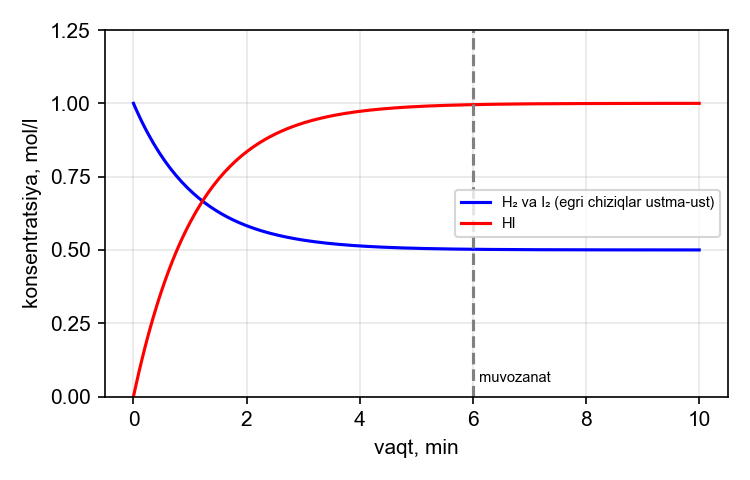
\includegraphics[width=0.86\linewidth]{rasmlar/g_muvozanat.png}\end{center}
Grafikdan foydalanib, muvozanat \textbf{konstantasini (K) aniqlang.}

\noindent A)~\textsl{2} \hfill B)~\textsl{8} \hfill C)~\textsl{4} \hfill D)~\textsl{1}\par
\vspace{4pt}
\end{multicols}
\noindent\textbf{9.} Tuzning eruvchanligi (g/100 g suv) haroratga bog`liq jadvalda berilgan:
\begin{center}
\renewcommand{\arraystretch}{1.15}
\begin{tabular}{|c|c|c|c|c|c|c|c|}\hline
\textbf{T, \textdegree{}C} & \textbf{0} & \textbf{10} & \textbf{20} & \textbf{30} & \textbf{40} & \textbf{50} & \textbf{60} \\ \hline
S & 13 & 20 & 30 & 45 & 62 & 80 & 102 \\ \hline
\end{tabular}
\end{center}
50 \textdegree{}C da tayyorlangan to`yingan eritmaning 180 g i 20 \textdegree{}C gacha sovitilganda necha gramm tuz cho`kmaga tushadi?

\noindent A)~\textsl{30} \hfill B)~\textsl{50} \hfill C)~\textsl{80} \hfill D)~\textsl{20}\par
\vspace{4pt}
\begin{multicols}{2}
\noindent\textbf{10.} pH = 12 bo`lgan NaOH eritmasining 200 ml siga necha ml suv qo`shilsa, eritma pH = 11 ga teng bo`ladi?

\noindent A)~\textsl{1800} \hfill B)~\textsl{1000} \hfill C)~\textsl{2000} \hfill D)~\textsl{900}\par
\vspace{4pt}
\noindent\textbf{11.} N\textsubscript{2} + 3H\textsubscript{2} $\rightleftarrows$ 2NH\textsubscript{3} + Q reaksiyasi doimiy hajmli idishda muvozanatga keltirilgandan so`ng harorat tushirildi. Yangi muvozanat qaror topgunga qadar sistemadagi moddalar konsentratsiyasi qanday o`zgaradi?
\noindent A)~\textsl{N\textsubscript{2} ortadi, H\textsubscript{2} ortadi, NH\textsubscript{3} kamayadi}\par
\noindent B)~\textsl{N\textsubscript{2} kamayadi, H\textsubscript{2} kamayadi, NH\textsubscript{3} kamayadi}\par
\noindent C)~\textsl{N\textsubscript{2} ortadi, H\textsubscript{2} kamayadi, NH\textsubscript{3} ortadi}\par
\noindent D)~\textsl{N\textsubscript{2} kamayadi, H\textsubscript{2} kamayadi, NH\textsubscript{3} ortadi}\par
\vspace{4pt}
\noindent\textbf{12.} KMnO\textsubscript{4} + HCl $\to$ MnCl\textsubscript{2} + Cl\textsubscript{2} + KCl + H\textsubscript{2}O reaksiya \textbf{tenglamasini tenglang.} 3 mol KMnO\textsubscript{4} to`liq reaksiyaga kirishganda qaytaruvchi vazifasini bajargan HCl miqdori necha mol?

\noindent A)~\textsl{24} \hfill B)~\textsl{30} \hfill C)~\textsl{9} \hfill D)~\textsl{15}\par
\vspace{4pt}
\noindent\textbf{13.} CuSO\textsubscript{4} eritmasi inert elektrodlar yordamida 5 A tok kuchi bilan 1930 s elektroliz qilindi. Anodda ajralgan gazning \textbf{hajmini (l, n.sh.) aniqlang.}

\noindent A)~\textsl{0,56} \hfill B)~\textsl{0,28} \hfill C)~\textsl{1,12} \hfill D)~\textsl{2,24}\par
\vspace{4pt}
\noindent\textbf{14.} Quyidagi jarayonlardan qaysilarida oltingugurt(IV) oksid hosil bo`ladi? 1) FeS\textsubscript{2} ning havoda yonishi; 2) Cu ning konsentrlangan H\textsubscript{2}SO\textsubscript{4} bilan qizdirilishi; 3) Zn ning suyultirilgan H\textsubscript{2}SO\textsubscript{4} bilan reaksiyasi; 4) oltingugurtning yonishi

\noindent A)~\textsl{1, 3, 4} \hfill B)~\textsl{1, 2, 4} \hfill C)~\textsl{2, 3, 4} \hfill D)~\textsl{1, 2, 3}\par
\vspace{4pt}
\noindent\textbf{15.} 5,6 l (n.sh.) ammiakdan ketma-ket oksidlash (NO $\to$ NO\textsubscript{2}) va NO\textsubscript{2} ni suv hamda kislorod bilan yutish orqali nitrat kislota olindi. Umumiy unum 80\% bo`lsa, hosil bo`lgan kislotadan tayyorlanadigan 63\% li eritmaning \textbf{massasini (g) aniqlang.}

\noindent A)~\textsl{12,5} \hfill B)~\textsl{25} \hfill C)~\textsl{31,5} \hfill D)~\textsl{20}\par
\vspace{4pt}
\noindent\textbf{16.} Mis va temirdan iborat 12 g aralashmaga sovuq konsentrlangan nitrat kislota ta'sir ettirilganda 4,48 l (n.sh.) gaz ajraldi. Reaksiyaga kirishmay qolgan qoldiq suyultirilgan xlorid kislotada eritilganda ajraladigan gazning \textbf{hajmini (l, n.sh.) aniqlang.}

\noindent A)~\textsl{1,12} \hfill B)~\textsl{2,24} \hfill C)~\textsl{3,36} \hfill D)~\textsl{4,48}\par
\vspace{4pt}
\noindent\textbf{17.} 0,1 mol Cu(NO\textsubscript{3})\textsubscript{2} va 0,2 mol NaNO\textsubscript{3} dan iborat aralashma to`liq parchalanguncha qizdirildi (mis nitrat oksidgacha, natriy nitrat nitritgacha parchalanadi). Qattiq qoldiq \textbf{massasini (g) aniqlang.}

\noindent A)~\textsl{17,8} \hfill B)~\textsl{25,6} \hfill C)~\textsl{21,8} \hfill D)~\textsl{8,0}\par
\vspace{4pt}
\noindent\textbf{18.} Alyuminiy va mis aralashmasining 10 g massasi mo`l NaOH eritmasida eritilganda 6,72 l (n.sh.) gaz ajraldi. Aralashmada mis massa ulushi necha foiz?

\noindent A)~\textsl{46} \hfill B)~\textsl{54} \hfill C)~\textsl{27} \hfill D)~\textsl{64}\par
\vspace{4pt}
\noindent\textbf{19.} Natriy va kaliyning teng mol nisbatdagi aralashmasi suv bilan reaksiyaga kirishib, 5,6 l (n.sh.) vodorod hosil qildi. Aralashma \textbf{massasini (g) aniqlang.}

\noindent A)~\textsl{11,5} \hfill B)~\textsl{19,5} \hfill C)~\textsl{15,5} \hfill D)~\textsl{7,75}\par
\vspace{4pt}
\noindent\textbf{20.} CH\textsubscript{3}--CH(CH\textsubscript{3})--CH(C\textsubscript{2}H\textsubscript{5})--CH\textsubscript{2}--CH\textsubscript{3} uglevodorodni sistematik nomenklatura bo`yicha \textbf{nomlang.}

\noindent\begin{tabular}{@{}p{0.47\linewidth}@{}p{0.47\linewidth}@{}}
A)~\textsl{2-metil-3-etilpentan} & B)~\textsl{2,3-dietilbutan} \\
C)~\textsl{3-etil-2-metilpentan} & D)~\textsl{3-izopropilpentan} \\
\end{tabular}\par
\vspace{4pt}
\noindent\textbf{21.} Atsetilen va etilendan iborat 0,4 mol aralashma tarkibida 96 g brom bo`lgan bromli suv bilan to`liq reaksiyaga kirishdi. Dastlabki aralashmaning \textbf{massasini (g) aniqlang.}

\noindent A)~\textsl{11,2} \hfill B)~\textsl{9,6} \hfill C)~\textsl{12} \hfill D)~\textsl{10,8}\par
\vspace{4pt}
\noindent\textbf{22.} Etanal va propanondan iborat 10,2 g aralashma Ag\textsubscript{2}O ning ammiakli eritmasi (mo`l) bilan qizdirilganda 21,6 g kumush ajraldi. Aralashmadagi propanon \textbf{massasini (g) aniqlang.}

\noindent A)~\textsl{2,9} \hfill B)~\textsl{5,8} \hfill C)~\textsl{4,4} \hfill D)~\textsl{8,7}\par
\vspace{4pt}
\noindent\textbf{23.} Benzol va toluoldan iborat 62 g aralashma kaliy permanganatning sulfat kislotali eritmasi bilan oksidlanganda 30,5 g benzoy kislota hosil bo`ldi. Dastlabki aralashmaning umumiy modda \textbf{miqdorini (mol) aniqlang.}

\noindent A)~\textsl{0,5} \hfill B)~\textsl{0,6} \hfill C)~\textsl{0,9} \hfill D)~\textsl{0,75}\par
\vspace{4pt}
\noindent\textbf{24.} Metanol va etanoldan iborat 7,8 g aralashma natriy bilan to`liq reaksiyaga kirishganda 2,24 l (n.sh.) vodorod ajraldi. Aralashmadagi metanol \textbf{massasini (g) aniqlang.}

\noindent A)~\textsl{3,2} \hfill B)~\textsl{4,6} \hfill C)~\textsl{1,6} \hfill D)~\textsl{6,4}\par
\vspace{4pt}
\noindent\textbf{25.} Metilamin va etilamindan iborat 0,3 mol aralashma kislorodda to`liq yondirilganda 0,4 mol karbonat angidrid hosil bo`ldi. Yonish uchun sarflangan kislorodning \textbf{hajmini (l, n.sh.) aniqlang.}

\noindent A)~\textsl{16,8} \hfill B)~\textsl{14,56} \hfill C)~\textsl{18,48} \hfill D)~\textsl{20,16}\par
\vspace{4pt}
\noindent\textbf{26.} Chumoli va sirka kislotalarning teng mol miqdordagi 10,6 g aralashmasiga Ag\textsubscript{2}O ning ammiakli eritmasi mo`l miqdorda qo`shilib qizdirildi. Hosil bo`lgan cho`kma \textbf{massasini (g) aniqlang.}

\noindent A)~\textsl{10,8} \hfill B)~\textsl{21,6} \hfill C)~\textsl{43,2} \hfill D)~\textsl{32,4}\par
\vspace{4pt}
\noindent\textbf{27.} Tabiiy kauchukning polimerlanish darajasi 2500 bo`lsa, shu kauchukning 340 g massasida nechta makromolekula bor? (N\textsubscript{A} = 6$\cdot$10\textsuperscript{23})

\noindent A)~\textsl{1,2$\cdot$10\textsuperscript{21}} \hfill B)~\textsl{1,2$\cdot$10\textsuperscript{22}} \hfill C)~\textsl{2,4$\cdot$10\textsuperscript{21}} \hfill D)~\textsl{6$\cdot$10\textsuperscript{20}}\par
\vspace{4pt}
\noindent\textbf{28.} Maltoza va saxarozadan iborat 855 g aralashma gidrolizlandi. Hosil bo`lgan moddalar bilan "kumush ko`zgu" reaksiyasi o`tkazilganda 756 g kumush ajraldi (faqat glyukoza ishtirok etadi). Aralashmadagi maltoza \textbf{massasini (g) aniqlang.}

\noindent A)~\textsl{171} \hfill B)~\textsl{513} \hfill C)~\textsl{684} \hfill D)~\textsl{342}\par
\vspace{4pt}
\noindent\textbf{29.} 806 g tripalmitin natriy ishqori bilan to`liq gidrolizlanganda necha gramm sovun hosil bo`ladi?

\noindent A)~\textsl{556} \hfill B)~\textsl{918} \hfill C)~\textsl{834} \hfill D)~\textsl{278}\par
\vspace{4pt}
\noindent\textbf{30.} Rasmda laboratoriyada etilen olish tajribasi tasvirlangan. Ajralgan gaz bromli suvga va KMnO\textsubscript{4} eritmasiga yuttirildi hamda yondirildi. Qaysi kuzatuvlar to`g`ri?
\begin{center}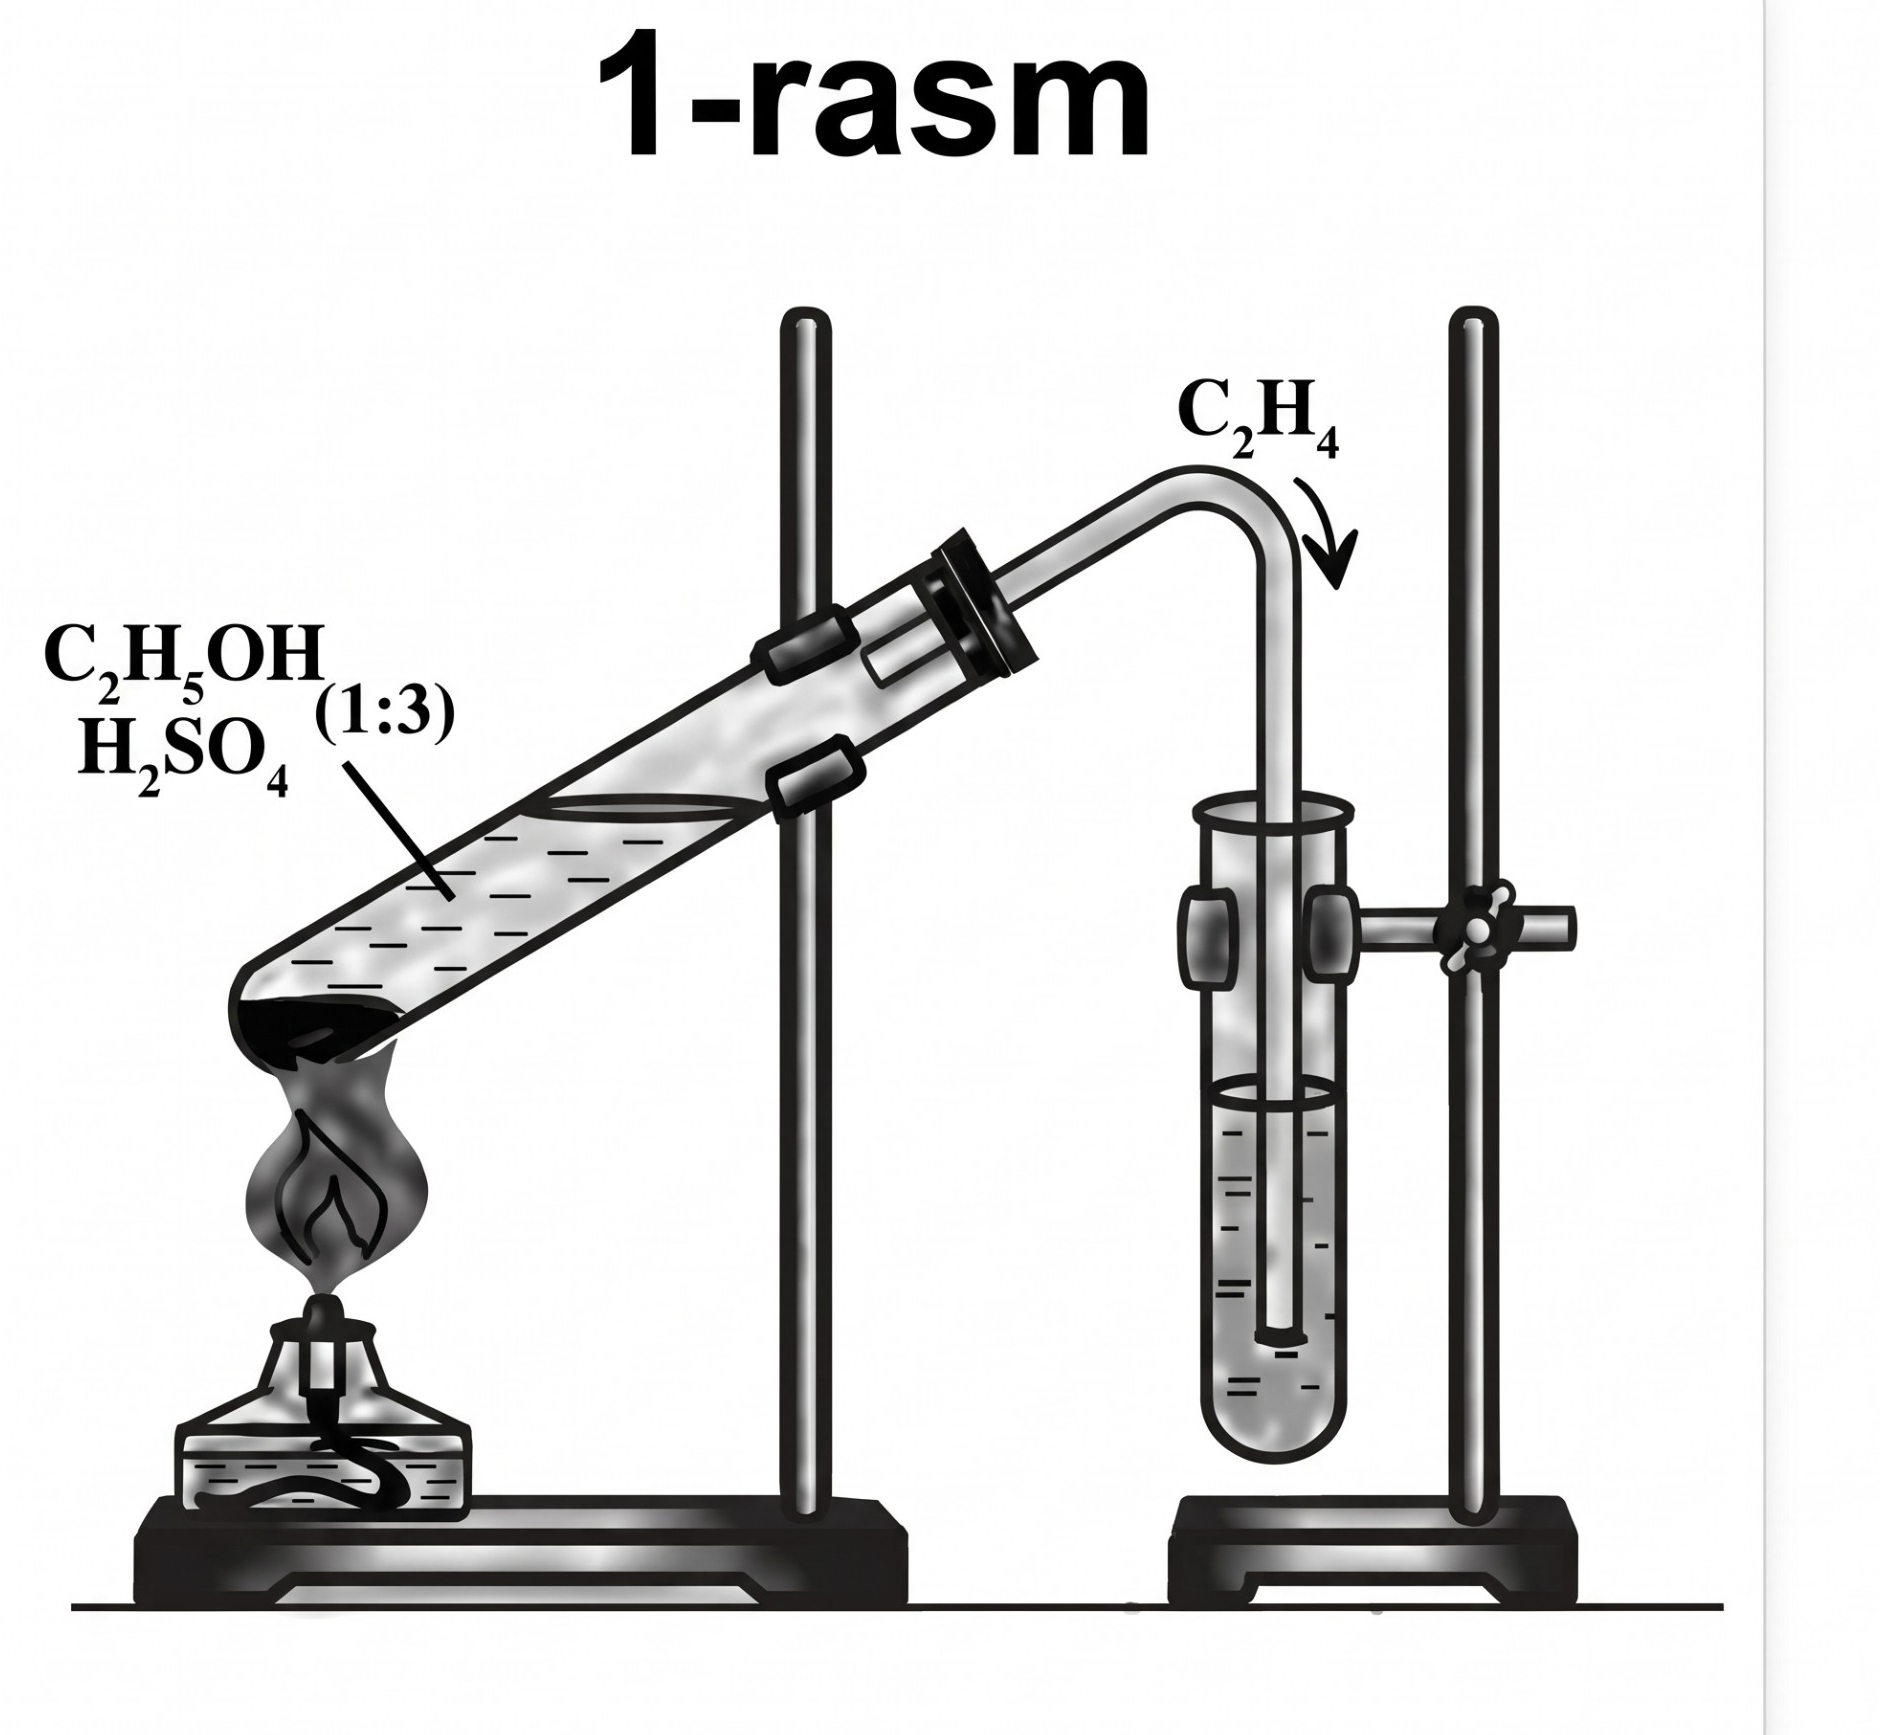
\includegraphics[width=0.86\linewidth]{rasmlar/lab_etilen.png}\end{center}
1) bromli suv rangsizlanadi; 2) KMnO\textsubscript{4} eritmasi rangsizlanadi; 3) gaz havorang alanga bilan yonadi; 4) gaz qurumli, tutaydigan alanga bilan yonadi

\noindent A)~\textsl{1, 2, 4} \hfill B)~\textsl{2, 3, 4} \hfill C)~\textsl{1, 3, 4} \hfill D)~\textsl{1, 2, 3}\par
\vspace{4pt}
\noindent\textbf{31.} Qaysi gazni ham suvni siqib chiqarish, ham havoni siqib chiqarish usulida to`plash mumkin?

\noindent A)~\textsl{H\textsubscript{2}} \hfill B)~\textsl{NO\textsubscript{2}} \hfill C)~\textsl{NH\textsubscript{3}} \hfill D)~\textsl{O\textsubscript{2}}\par
\vspace{4pt}
\noindent\textbf{32.} Aralashmalarni ularni ajratish usullari bilan moslang. 1) suv va etanol aralashmasi; 2) qum va suv aralashmasi; 3) suv va kerosin aralashmasi; 4) osh tuzi eritmasi. a) distillash;  b) filtrlash;  c) bo`lgich voronka;  d) bug`latish.
\noindent A)~\textsl{1-b, 2-a, 3-c, 4-d}\par
\noindent B)~\textsl{1-a, 2-b, 3-c, 4-d}\par
\noindent C)~\textsl{1-a, 2-b, 3-d, 4-c}\par
\noindent D)~\textsl{1-c, 2-b, 3-a, 4-d  ---}\par
\vspace{4pt}
\end{multicols}
\medskip
\noindent\setlength{\fboxsep}{0pt}\fbox{\begin{tabular}{p{0.74\linewidth}|p{0.2\linewidth}}
\parbox[t]{0.72\linewidth}{\vspace{3pt}\textbf{Topshiriqlar (33--35) va javob variant (A--F)larini o`zaro to`g`ri moslashtiring.} 400 g 16\% li mis(II)-sulfat eritmasiga temir plastinka tushirildi. Birmuncha vaqt o`tgach plastinka eritmadan chiqarib olindi; uning massasi 1,6 g ga ortgan edi. Eritmada qolgan CuSO\textsubscript{4} keyin inert elektrodlar yordamida to`liq elektroliz qilindi (tok kuchi 10 A).
\vspace{3pt}} & \parbox[t]{0.19\linewidth}{\vspace{3pt}A~\textsl{3860}\\[3pt]
B~\textsl{11,2}\\[3pt]
C~\textsl{12,8}\\[3pt]
D~\textsl{1,6}\\[3pt]
E~\textsl{398,4}\\[3pt]
F~\textsl{7720}}\\ \hline
\parbox[t]{0.72\linewidth}{\vspace{2pt}\textbf{33. Plastinka sirtida ajralgan mis massasini (g) aniqlang.}\vspace{2pt}} & \\ \hline
\parbox[t]{0.72\linewidth}{\vspace{2pt}\textbf{34. Plastinka chiqarib olingach, eritmaning massasini (g) aniqlang.}\vspace{2pt}} & \\ \hline
\parbox[t]{0.72\linewidth}{\vspace{2pt}\textbf{35. Eritmada qolgan CuSO\textsubscript{4} ni to`liq elektroliz qilish uchun necha sekund kerak?}\vspace{2pt}} & 
\end{tabular}}
\par\bigskip
\noindent\textbf{36.} FeCl\textsubscript{2} + KMnO\textsubscript{4} + HCl $\to$ FeCl\textsubscript{3} + MnCl\textsubscript{2} + KCl + H\textsubscript{2}O reaksiya tenglamasini eng kichik butun sonlarda tenglang va barcha koeffitsiyentlar \textbf{yig`indisini aniqlang.}
\javob
\noindent\textbf{37.} 25 g mis kuporosi (CuSO\textsubscript{4}$\cdot$5H\textsubscript{2}O) 175 g suvda eritildi. Hosil bo`lgan eritma inert elektrodlar yordamida 5 A tok kuchi bilan 1930 s elektroliz qilindi. Elektroliz tugagach, eritmadagi sulfat kislotaning massa \textbf{ulushini (\%) aniqlang.}
\javob
\noindent\textbf{38.} Alyuminiy va alyuminiy oksididan iborat 7,8 g aralashma mo`l xlorid kislotada eritilganda 3,36 l (n.sh.) vodorod ajraldi. Hosil bo`lgan eritmaga mo`l miqdorda ammiak eritmasi qo`shildi, cho`kma ajratilib, to`liq qizdirildi. Qoldiq \textbf{massasini (g) aniqlang.}
\javob
\noindent\textbf{39.} 0,2 mol noma'lum alkinni to`liq yoqish uchun 17,92 l (n.sh.) kislorod sarflandi. Shu alkin Kucherov reaksiyasi bo`yicha gidratlanganda (unum 50\%) hosil bo`ladigan moddaning \textbf{massasini (g) aniqlang.}
\javob
\noindent\textbf{40.} To`yingan monokarbon kislotaning natriyli tuzi mo`l NaOH bilan qizdirilganda 2,24 l (n.sh.) gaz va 10,6 g Na\textsubscript{2}CO\textsubscript{3} hosil bo`ldi. Hosil bo`lgan gazning vodorodga nisbatan zichligi 22 ga teng. Dastlabki karbon kislotaning molyar \textbf{massasini (g/mol) aniqlang.}
\javob
\par\bigskip\begin{center}\textbf{\fontsize{13}{15}\selectfont YOZMA ISH}\end{center}
\noindent\textbf{41.} \textbf{Topshiriqni bajarish jarayonida barcha reaksiya tenglamalarini yozing. Miqdoriy va arifmetik hisoblashlarni (unga asos bo`lgan usul yoki formulani ko`rsatgan holda) uzviy ketma-ketlikda bajaring.}\par\smallskip
75 g pirit rudasi (tarkibida 80\% FeS\textsubscript{2}) havoda to`liq yondirildi. Hosil bo`lgan oltingugurt(IV) oksidning hammasi hajmi 2 l bo`lgan idishga 0,8 mol kislorod bilan kiritildi va katalizator ishtirokida qizdirildi. SO\textsubscript{2} ning 60\% i reaksiyaga kirishganda sistema muvozanat holatiga keldi: 2SO\textsubscript{2} + O\textsubscript{2} $\rightleftarrows$ 2SO\textsubscript{3}. Hosil bo`lgan SO\textsubscript{3} ning hammasi 352 g suvda eritildi.\par
\noindent 1)Ruda yonganda hosil bo`lgan SO\textsubscript{2} ning hajmini (l, n.sh.) va qattiq qoldiq (Fe\textsubscript{2}O\textsubscript{3}) massasini (g) hisoblang.\par
\noindent 2)Muvozanat konstantasini (K) hisoblang.\par
\noindent 3)Hosil bo`lgan sulfat kislota eritmasining massa ulushini (\%) aniqlang.\par
\noindent 4)Shu eritmani to`liq neytrallash uchun zichligi 1,25 g/ml bo`lgan 20\% li NaOH eritmasidan necha ml kerak?\par
\diqqat{Mazkur topshiriq kengaytirilgan javobni talab etib, uning yechilish usuli va shu usul asosidagi barcha hisoblash amallari javoblar varaqasida aks etishi lozim.}
\noindent\textbf{42.} Reaksiya tenglamalarini tugallang va tenglang. Hosil bo`lgan organik moddalarning tuzilish formulalarini yozing va ularni nomlang.\par
\noindent 1)CH\textsubscript{3}COONa + NaOH $\xrightarrow{\text{t}}$\par
\noindent 2)CH\textsubscript{3}--CH=CH\textsubscript{2} + HBr $\to$\par
\noindent 3)n CH\textsubscript{2}=CH--CH=CH\textsubscript{2} $\to$ (1,4-birikish)\par
\noindent 4)C\textsubscript{6}H\textsubscript{5}--CH\textsubscript{3} + KMnO\textsubscript{4} + H\textsubscript{2}SO\textsubscript{4} $\to$\par
\noindent 5)CH\textsubscript{3}--CHO + Ag\textsubscript{2}O $\xrightarrow{\text{NH\textsubscript{3}, t}}$\par
\noindent 6)C\textsubscript{6}H\textsubscript{5}OH + Br\textsubscript{2} (mo`l, bromli suv) $\to$\par
\noindent 7)H\textsubscript{2}N--CH\textsubscript{2}--COOH + HCl $\to$\par
\diqqat{Mazkur topshiriq kengaytirilgan javobni talab etib, uning yechilish usuli va shu usul asosidagi barcha hisoblash amallari javoblar varaqasida aks etishi lozim.}
\noindent\textbf{43.} \textbf{Topshiriqni bajarish jarayonida barcha reaksiya tenglamalarini yozing. Miqdoriy va arifmetik hisoblashlarni (unga asos bo`lgan usul yoki formulani ko`rsatgan holda) uzviy ketma-ketlikda bajaring.}\par\smallskip
Laboratoriyada 1--4-raqamli probirkalarda tartibsiz holda glyukoza, kraxmal kleysteri, tuxum oqsili va glitserin eritmalari bor. Ularni aniqlash uchun quyidagi tajribalar o`tkazildi:\par
a) 1-probirkaga yodning spirtdagi eritmasidan qo`shildi --- eritma ko`k rangga bo`yaldi.\par
b) 2-probirkaga ishqor eritmasi va bir necha tomchi mis(II)-sulfat qo`shilganda eritma qizil-binafsha rangga bo`yaldi; boshqa porsiyasiga konsentrlangan HNO\textsubscript{3} qo`shib qizdirilganda sariq rang paydo bo`ldi.\par
c) 3- va 4-probirkalarga yangi cho`ktirilgan Cu(OH)\textsubscript{2} qo`shilganda ikkalasida ham cho`kma erib, ko`k eritma hosil bo`ldi. 3-probirka qizdirilganda avval sariq, so`ng qizil cho`kma tushdi, 4-probirkada esa o`zgarish bo`lmadi.\par
\noindent 1)Kuzatilgan reaksiyalardan "kumush ko`zgu"ga o`xshash glyukozaning Cu(OH)\textsubscript{2} bilan reaksiya tenglamasini yozing. 18 g glyukoza mo`l Cu(OH)\textsubscript{2} bilan qizdirilganda hosil bo`lgan qizil cho`kmaning massasini (g) hisoblang.\par
\noindent 2)1--4-probirkalardagi moddalarni aniqlang (probirka raqami bilan moslab yozing).\par
\noindent 3)a), b) va c) bo`yicha kuzatilgan rang o`zgarishlarining sababini tushuntiring: qaysi funksional guruh yoki bog` bilan bog`liq?\par
\noindent 4)Tajribada probirkani qizdirish va konsentrlangan HNO\textsubscript{3} bilan ishlashda qanday xavfsizlik qoidalariga rioya qilish kerak? Kamida uchta qoidani yozing.\par
\diqqat{Mazkur topshiriq kengaytirilgan javobni talab etib, uning yechilish usuli va shu usul asosidagi barcha hisoblash amallari javoblar varaqasida aks etishi lozim.}
\newpage
\noindent\textbf{\fontsize{13}{15}\selectfont Nazorat testi}\ \textit{$\cdot$ 1-variant}\hfill \textbf{Javoblar kaliti}\par\smallskip\hrule\smallskip
\textit{Faqat o`qituvchi uchun.}\par\medskip
\noindent\textbf{1--32-savollar}\par\smallskip
\noindent\begin{tabular}{|c|c|c|c|c|c|c|c|c|c|c|c|c|c|c|c|}\hline
\textbf{1} & \textbf{2} & \textbf{3} & \textbf{4} & \textbf{5} & \textbf{6} & \textbf{7} & \textbf{8} & \textbf{9} & \textbf{10} & \textbf{11} & \textbf{12} & \textbf{13} & \textbf{14} & \textbf{15} & \textbf{16}\\\hline
\textsl{B} & \textsl{B} & \textsl{C} & \textsl{B} & \textsl{C} & \textsl{B} & \textsl{A} & \textsl{C} & \textsl{B} & \textsl{A} & \textsl{D} & \textsl{D} & \textsl{A} & \textsl{B} & \textsl{D} & \textsl{B}\\\hline
\textbf{17} & \textbf{18} & \textbf{19} & \textbf{20} & \textbf{21} & \textbf{22} & \textbf{23} & \textbf{24} & \textbf{25} & \textbf{26} & \textbf{27} & \textbf{28} & \textbf{29} & \textbf{30} & \textbf{31} & \textbf{32}\\\hline
\textsl{C} & \textsl{A} & \textsl{C} & \textsl{C} & \textsl{D} & \textsl{B} & \textsl{D} & \textsl{A} & \textsl{C} & \textsl{B} & \textsl{A} & \textsl{D} & \textsl{C} & \textsl{D} & \textsl{D} & \textsl{B}\\\hline
\end{tabular}\par\medskip
\noindent\textbf{33--35-savollar}\par\smallskip
\noindent\begin{tabular}{|c|c|c|}\hline \textbf{No} & \textbf{Javob} & \textbf{Qiymat}\\\hline
33 & \textsl{C} & 12,8\\\hline
34 & \textsl{E} & 398,4\\\hline
35 & \textsl{A} & 3860\\\hline
\end{tabular}\par\medskip
\noindent\textbf{36--40-savollar}\par\smallskip
\noindent\begin{tabular}{|c|c|}\hline \textbf{No} & \textbf{To`g`ri javob}\\\hline
36 & 25\\\hline
37 & 2,5\\\hline
38 & 10,2\\\hline
39 & 5,8\\\hline
40 & 88\\\hline
\end{tabular}\par\medskip
\noindent\textbf{41--43-topshiriqlar: qisqa yechim}\par\smallskip
\noindent\textbf{41-topshiriq.}\par
\noindent 1) FeS\textsubscript{2}: 75 $\cdot$ 0,8 = 60 g = 0,5 mol (M = 120). 4FeS\textsubscript{2} + 11O\textsubscript{2} $\to$ 2Fe\textsubscript{2}O\textsubscript{3} + 8SO\textsubscript{2}: n(SO\textsubscript{2}) = 1 mol $\to$ \textbf{22,4 l}; n(Fe\textsubscript{2}O\textsubscript{3}) = 0,25 mol $\to$ 0,25 $\cdot$ 160 = \textbf{40 g}.\par
\noindent 2) SO\textsubscript{2} reaksiyaga kirgan: 0,6 mol $\to$ SO\textsubscript{3} 0,6 mol; O\textsubscript{2} sarfi 0,3 mol. Muvozanatda: SO\textsubscript{2} 0,4; O\textsubscript{2} 0,5; SO\textsubscript{3} 0,6 mol $\to$ konsentratsiyalar (\textit{V} = 2 l): 0,2; 0,25; 0,3 mol/l. K = [SO\textsubscript{3}]\textsuperscript{2}/([SO\textsubscript{2}]\textsuperscript{2}$\cdot$[O\textsubscript{2}]) = 0,09/(0,04 $\cdot$ 0,25) = \textbf{9}.\par
\noindent 3) SO\textsubscript{3} + H\textsubscript{2}O $\to$ H\textsubscript{2}SO\textsubscript{4}: 0,6 mol = 58,8 g; eritma 0,6 $\cdot$ 80 + 352 = 400 g $\to$ $\omega$ = 58,8/400 = \textbf{14,7\%}.\par
\noindent 4) H\textsubscript{2}SO\textsubscript{4} + 2NaOH $\to$ Na\textsubscript{2}SO\textsubscript{4} + 2H\textsubscript{2}O: NaOH 1,2 mol = 48 g; eritma 48/0,2 = 240 g; \textit{V} = 240/1,25 = \textbf{192 ml}.\par
\noindent Jami: M 14 + A 11 = 25 ball.\par
\noindent\textbf{42-topshiriq.}\par
\noindent 1) (4 ball) CH\textsubscript{3}COONa + NaOH $\xrightarrow{\text{t}}$ CH\textsubscript{4} + Na\textsubscript{2}CO\textsubscript{3} --- metan.\par
\noindent 2) (4 ball) CH\textsubscript{3}--CH=CH\textsubscript{2} + HBr $\to$ CH\textsubscript{3}--CHBr--CH\textsubscript{3} --- 2-brompropan (Markovnikov qoidasi).\par
\noindent 3) (3 ball) n CH\textsubscript{2}=CH--CH=CH\textsubscript{2} $\to$ (--CH\textsubscript{2}--CH=CH--CH\textsubscript{2}--)n --- polibutadiyen (butadiyen kauchuk).\par
\noindent 4) (5 ball) 5C\textsubscript{6}H\textsubscript{5}--CH\textsubscript{3} + 6KMnO\textsubscript{4} + 9H\textsubscript{2}SO\textsubscript{4} $\to$ 5C\textsubscript{6}H\textsubscript{5}--COOH + 6MnSO\textsubscript{4} + 3K\textsubscript{2}SO\textsubscript{4} + 14H\textsubscript{2}O --- benzoy kislota.\par
\noindent 5) (3 ball) CH\textsubscript{3}--CHO + Ag\textsubscript{2}O $\xrightarrow{\text{NH\textsubscript{3}, t}}$ CH\textsubscript{3}--COOH + 2Ag$\downarrow$ --- etan (sirka) kislota.\par
\noindent 6) (3 ball) C\textsubscript{6}H\textsubscript{5}OH + 3Br\textsubscript{2} $\to$ C\textsubscript{6}H\textsubscript{2}Br\textsubscript{3}OH$\downarrow$ + 3HBr --- 2,4,6-tribromfenol (oq cho`kma).\par
\noindent 7) (3 ball) H\textsubscript{2}N--CH\textsubscript{2}--COOH + HCl $\to$ [H\textsubscript{3}N\textsuperscript{+}--CH\textsubscript{2}--COOH]Cl\textsuperscript{$-$} --- glitsinning xlorid kislotali tuzi.\par
\noindent Jami 4+4+3+5+3+3+3 = 25 ball.\par
\noindent\textbf{43-topshiriq.}\par
\noindent 2) 1 --- kraxmal kleysteri (yod bilan ko`k rang); 2 --- tuxum oqsili (biuret va ksantoprotein reaksiyalari); 3 --- glyukoza; 4 --- glitserin.\par
\noindent 1) CH\textsubscript{2}OH--(CHOH)\textsubscript{4}--CHO + 2Cu(OH)\textsubscript{2} $\to$ CH\textsubscript{2}OH--(CHOH)\textsubscript{4}--COOH + Cu\textsubscript{2}O$\downarrow$ + 2H\textsubscript{2}O. n(glyukoza) = 18/180 = 0,1 mol $\to$ n(Cu\textsubscript{2}O) = 0,1 mol $\to$ m = 0,1 $\cdot$ 144 = \textbf{14,4 g}.\par
\noindent 3) a) kraxmal yod bilan ko`k rang beradi (kraxmalning sifat reaksiyasi). b) oqsil: ishqoriy muhitda CuSO\textsubscript{4} bilan qizil-binafsha rang --- peptid bog` (--CO--NH--) uchun biuret reaksiyasi; konsentrlangan HNO\textsubscript{3} bilan sariq rang --- aromatik halqali aminokislota qoldiqlari (ksantoprotein reaksiya). c) glyukoza va glitserin Cu(OH)\textsubscript{2} ni eritib, ko`k kompleks hosil qiladi (ko`p atomli spirt guruhlari); faqat glyukozada aldegid guruh bor, shuning uchun qizdirilganda Cu(OH)\textsubscript{2} Cu\textsubscript{2}O (sariq CuOH, so`ng qizil Cu\textsubscript{2}O) gacha qaytariladi; glitserin aldegid guruhga ega emas.\par
\noindent 4) Misol qoidalar: probirka qisqichda tik, og`zi o`zingizga va boshqalarga qaratilmagan holda ohista qizdiriladi; konsentrlangan kislotani ehtiyotlik bilan, ko`zoynak va qo`lqopda ishlatish, teriga tushsa ko`p suv bilan yuvish; reaktivlarni tatib ko`rmaslik; ortiqcha reaktivni idishga qaytarmaslik; reaksiyalarni kichik miqdorda o`tkazish.\par
\noindent Baholash: M 10 + 4 + 7 + 2 = 23 ball, A 2 ball $\to$ 25 ball (kimyoviy tahlil jadvali: 4 band, M 23--25, A 1--2).\par
\end{document}
